\documentclass{scrartcl}

\usepackage{german}
\usepackage[utf8]{inputenc}  %Umlaute
\usepackage[T1]{fontenc}     %Umlauttrennung
\usepackage{lmodern}         %modernes Schriftbild
\usepackage{amsmath}         %math Umgebungen
\usepackage{graphicx}
\usepackage{hyperref}
\usepackage{graphicx}
\usepackage{gensymb}

\title{Physikpraktikum für Naturwissenschaftler \\ Versuch: Drehschwingungen}
\author{Felix Burr, Johannes Spindler (Gruppe 13)}
\date{Durchgeführt am 18. Oktober 2018}


\begin{document}
\begin{titlepage}
  \begin{center}
    \vspace*{1cm}
    \LARGE
    Physikpraktikum für Naturwissenschaftler \\
    \vspace*{1cm}
    \Huge
    \textbf{Versuch: Drehschwingungen} \\
    \vspace*{0.3cm}
    \Large
    Durchgeführt am 18. Oktober 2018 \\
    Betreuer: Christian Ganslmayer \\
    \vspace*{2.5cm}
    Gruppe 13 \\
    Felix Burr: felix.burr@uni-ulm.de \\
    Johannes Spindler: johannes.spindler@uni-ulm.de \\
    \vfill 
  \end{center}
  Wir bestätigen hiermit, das Protokoll selbstständig erarbeitet zu haben und in genauer Kenntnis über dessen Inhalt zu sein. \\
  \vspace*{0.8cm}
  \\
  Felix Burr
  \hfill
  Johannes Spindler
\end{titlepage}
\pagebreak
\tableofcontents


\pagebreak

\section{Einleitung}
Schwingungen sind uns aus vielfachen Alltagssituationen bekannt. Etwa beim Spielen eines Klaviers: Der Ton kommt durch das Schwingen der Saiten zustande und mithilfe der Pedale kann eine Dämpfung der Saitenschwingung eingestellt werden.
Auch in der Architektur müssen mögliche Schwingungen bedacht werden. Erdbeben und Sturm können starke erzwungene Schwingungen an Hochhäusern und Brücken verursachen. Im schlimmsten Fall, einer Resonanz zwischen Anregungs- und Systemfrequenz kommt es zu extremen Auslenkungen und Konstruktionen stürzen womöglich ein.
Deshalb werden wir uns in diesem Versuch mit Drehschwingungen beschäftigen, vor allem mit Dämpfung, erzwungener Schwingung und Resonanz.
\section{Versuch 1: Frequenz und Dämpfung der freien Schwingung}
\subsection{Versuchsdurchführung}
Wir verwenden für diesen Versuch ein Drehpendel. Dieses ist folgendermaßen aufgebaut: Ein  Kupferring und ein Hebel liegen drehbar auf einer Achse und sind miteinander durch eine Spiralfeder verbunden. Der Hebel kann von einem einstellbaren Motor periodisch ausgelenkt werden, was eine Schwingung des Kupferrades erzwingt.
Der Kupferring läuft außerdem durch die Polschuhe eines Elektromagneten, der als Wirbelstrombremse fungiert. Der Strom durch diesen kann eingestellt werden und abhängig von der Spulenspannung erfährt das Rad eine Dämpfung. Die Auslenkung des Rades kann an einer das Rad umrundenden Skala abgelesen werden.

Nun wird die Frequenz der freien Schwingung des Drehpendels ohne Dämpfung bestimmt. Dazu messen wir mit einer Stoppuhr, die Zeit, die das Pendel für 10 Perioden benötigt. Mit der Periodendauer $T$ können wir dann die Kreisfrequenz berechnen:
\begin{align*}
\omega = 2 \pi f = \dfrac{2 \pi}{T} 
\end{align*}

Im zweiten Teil des Versuchs wollen wir die Auswirkung der Dämpfungsspannung untersuchen. Wir führen also zwei Messreihen durch, einmal bei 2V Bremsspannung und einmal bei 4V. Wir messen jeweils den Maximalausschlag des Rades nach links in der ersten Periode, $x_{max}(1)$ [Skaleneinheiten SE], und denselben in der zweiten Periode, $x_{max}(2)$ [SE]. Damit können wir das logarithmische Dekrement $K$ bestimmen:
\begin{align*}
K = \dfrac{x_{max}(1)}{x_{max}(2)}
\end{align*}
$K$ benötigen wir um die Dämpfung $\beta$ [1/s] zu ermitteln:
\begin{align*}
e^{\beta T} = K \\
\beta = \dfrac{ln(k)}{T}
\end{align*}
Wir messen außerdem bei beiden Messreihen die Periode. Da die im Pendel eingebaute Zeitmessung mittels Lichtschranke nur Halbperioden messen kann, messen wir die linke und die rechte Halbperiode $T_{links}$ und $T_{rechts}$.
\subsection{Messwerte und Ergebnisse}
Die gemessenen Werte für die Periodendauer und für die Kreisfrequenz $\omega$ des Drehpendels ohne Dämpfung:
\begin{table}[h]
\begin{tabular}{l|l|l}
Messung    & $10 T$ {[}s{]} & $\omega$ {[}1/s{]}\\
\hline
1          & 19,75               & 3,18                  \\
2          & 19,81               & 3,17                  \\
3          & 19,87               & 3,16                  \\
4          & 19,62               & 3,20                  \\
5          & 19,78               & 3,18                  \\
Mittelwert & 19,77               & 3,18                 
\end{tabular}
\end{table}
\\
Die Messreihe zur Bestimmung der Dämpfungskonstante bei 2V Dämpfungsspannung:
\begin{table}[h]
\begin{tabular}{l|l|l|l|l|l|l|l}
Messung    & $x_{max}(1)$ [SE]      & $x_{max}(2)$ [SE]      & $T_{links}$ [s]      &      $T_{rechts}$ [s] & K [1]       & $\beta$ [1/s]     & $\omega$ [1/s]      \\
\hline
1          & 16,0 & 14,2  & 1,024 & 0,954 & 1,127 & 0,060 & 3,177 \\
2          & 16,0 & 14,4  & 1,024 & 0,954 & 1,111 & 0,053 & 3,177 \\
3          & 16,0 & 14,4  & 1,024 & 0,954 & 1,111 & 0,053 & 3,177 \\
4          & 16,0 & 14,2  & 1,024 & 0,954 & 1,127 & 0,060 & 3,177 \\
Mittelwert & 16,0 & 11,3  & 1,024 & 0,954 & 1,119 & 0,057 & 3,177
\end{tabular}
\end{table}
\\
Die Messreihe zur Bestimmung der Dämpfungskonstante bei 4V Dämpfungsspannung:
\begin{table}[h]
\begin{tabular}{l|l|l|l|l|l|l|l}
Messung    & $x_{max}(1)$ [SE]      & $x_{max}(2)$ [SE]      & $T_{links}$ [s]      &      $T_{rechts}$ [s] & K [1]       & $\beta$ [1/s]     & $\omega$ [1/s]      \\
\hline
1          & 16,0 & 11,0  & 1,025 & 0,955 & 1,455 & 0,189 & 3,173 \\
2          & 16,0 & 11,2  & 1,025 & 0,955 & 1,429 & 0,180 & 3,173 \\
3          & 16,0 & 11,2  & 1,025 & 0,955 & 1,429 & 0,180 & 3,173 \\
4          & 16,0 & 11,2  & 1,025 & 0,955 & 1,429 & 0,180 & 3,173 \\
Mittelwert & 16,0 & 11,15 & 1,025 & 0,955 & 1,435 & 0,182 & 3,173
\end{tabular}
\end{table}

\subsection{Fehlerrechnung}
\begin{align*}
\Delta \omega = \left| \dfrac{\partial \omega}{\partial T} \right| \Delta T = \left| - \dfrac{2 \pi}{T^{2}} \right| \Delta T = \dfrac{2 \pi}{T^{2}}  \Delta T
\end{align*}
\begin{align*}
\Delta K = \left| \dfrac{\partial K}{\partial x_{max}(1)} \right| \Delta x_{max}(1) + \left| \dfrac{\partial K}{\partial x_{max}(2)} \right| \Delta x_{max}(2) = \dfrac{1}{x_{max}(2)} \Delta x_{max}(1) + \dfrac{x_{max}(1)}{(x_{max}(2))^2} \Delta x_{max}(2)
\end{align*}
\begin{align*}
\Delta \beta = \left| \dfrac{\partial \beta}{\partial K} \right| \Delta K + \left| \dfrac{\partial \beta}{\partial T} \right| \Delta T = \left| \dfrac{1}{KT} \right| \Delta K + \left| - \dfrac{ln(K)}{T^2} \right| \Delta T = \dfrac{1}{KT} \Delta K + \dfrac{ln(K)}{T^2} \Delta T
\end{align*}
\subsection{Ergebnisdiskussion}
Wir können feststellen, dass die Dämpfung in unserem Experiment nur eine sehr kleine Änderung der Kreisfrequenz im Vergleich zur Kreisfrequenz der ungedämpften Schwingung hat. Das lässt sich mit folgender Formel erklären:
\begin{align*}
\omega = \sqrt{\omega_{0}^2 - \beta^2}
\end{align*}
$\omega_{0}$ ist hier die Eigenfrequenz des ungedämpften Systems, $\beta$ die Dämpfung und $\omega$ die Frequenz des gedämpften Systems. Da die Dämpfungskonstante in unseren Messungen nahe bei Null war und diese in der Formel im Quadrat steht, gilt:
\begin{align*}
\omega \approx \sqrt{\omega_{0}^2} = \omega_{0}
\end{align*}

\section{Versuch 2: Erzwungene Schwingungen}
\subsection{Versuchsdurchführung}
In diesem Versuch wird das Drehpendel von einem externen Motor erregt. Wir untersuchen
wie sich unterschiedliche Erregerfrequenzen auf das Pendel auswirken.

\begin{figure}[h]
  \caption{Drehpendel mit Erreger}
  \centering
    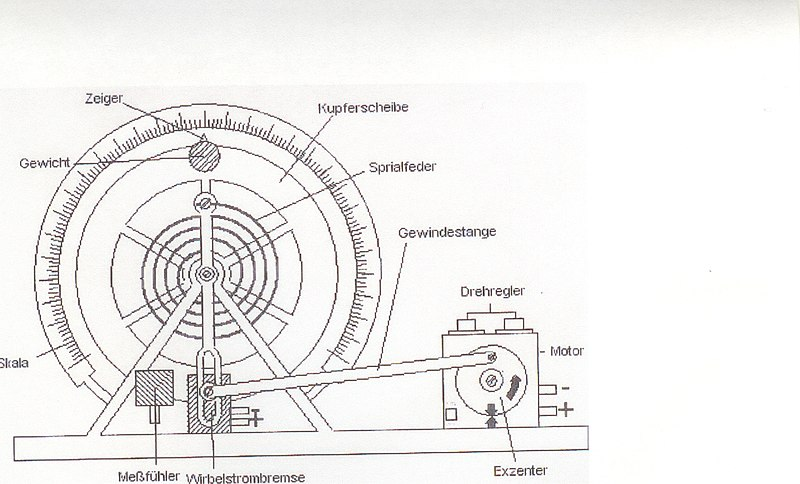
\includegraphics[width=0.75\textwidth]{800px-Pohlsches_Rad}
\end{figure}

In Versuch 2.1 haben wir durch probieren festgestellt, dass der optimale Phasenwinkel bei etwa 105$\degree$ liegt. 
\subsection{Messwerte und Ergebnisse}
Dämpfungsspannung von 2V:\\
\begin{tabular}{llllll}
Messung &F ($\frac{1}{10s}$)&Phasendifferenz ($ms$)&Phasendifferenz ($\degree$)&T ($ms$)&Amplitude ($cm$)\\\hline
1&40&145&24.1&2166&3.5\\
2&42&172&27.9&2216&6.5\\
3&43&295&49.6&2143&11\\
4&44&575&99.2&2086&15.2\\
5&45&945&176.0&1932&6.6\\
6&47&920&178.2&1859&2.9\\\\
\end{tabular}

Dämpfungsspannung von 4V:\\
\begin{tabular}{llllll}
Messung &F ($\frac{1}{10s}$)&Phasendifferenz ($ms$)&Phasendifferenz ($\degree$)&T ($ms$)&Amplitude ($cm$)\\\hline
1&40&312&51.8&2167&2.7\\
2&42&428&74.3&2073&3.9\\
3&43&523&93.0&2025&4.6\\
4&44&575&99.2&2086&15.2\\
5&45&625&113.5&1982&4\\
\end{tabular}
\subsection{Fehlerrechnung}

\subsection{Ergebnisdiskussion}



\section{Versuch 3: Computersimulation}
\subsection{Versuchsdurchführung}
Bei diesem Versuch verwenden wir eine MATLAB-Simulation, die die Phasenverschiebung nach Anregungsfrequenz und die Maximalamplitude nach Anregungsfrequenz bei einer erzwungenen Schwingung eines Federpendels zeigt. Die Anregungsfrequenz ist einstellbar, die Federhärte zufallsgeneriert und die Federmasse unbekannt. Wir wollen uns durch Probieren der Resonanzfrequenz des Pendels annähern.
Für den zweiten Teil des Versuchs verwenden wir die \\ Website http://wwwchem.uwimona.edu.jm/spectra/jsmol/demos/acetophenone.html, um den Zusammenhang zwischen den Molekülschwingungen und dem Infrarotspektrum des Acetophenon-Moleküls herzustellen.
\subsection{Ergebnisdiskussion}

\begin{figure}[h]
  \caption{Infrarotspektrum des Acetophenon-Moleküls}
  \centering
    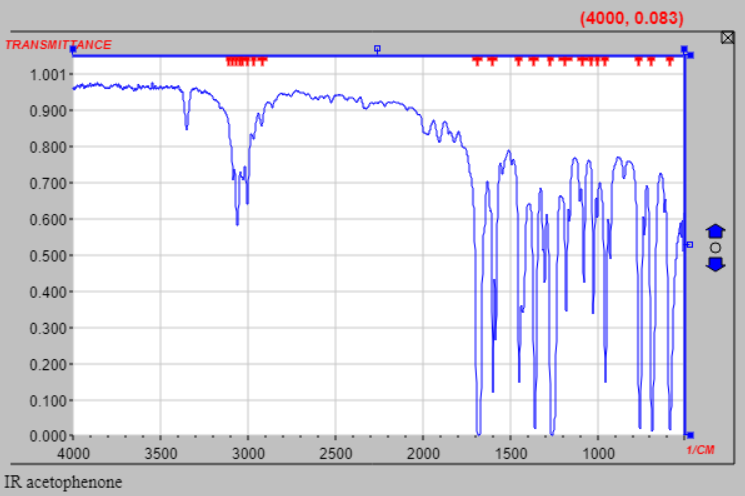
\includegraphics[width=0.75\textwidth]{acetophenon.png}
\end{figure}
Im Infrarotspektrum des Acetophenon-Moleküls erkennt man charakteristische Peaks nach unten. Das bedeutet, an diesen speziellen Strahlungsfrequenzen ist die Durchlässigkeit der Strahlung nahezu Null, aber benachbarte Frequenzen gewähren wieder eine hohe Durchlässigkeit. Hierbei handelt es sich um die Resonanzfrequenzen der Molekülbausteine, also kann an diesen Stellen des Spektrums besonders viel Strahlung absorbiert und gestreut werden. Es existieren mehrere solche Resonanzfrequenzen im Spektrum, da alle Kombinationen von Bindungen im Molekül schwingen können und das Molekül aus verschiedenen Atomen besteht.
\end{document}